\capitulo{5}{Aspectos relevantes del desarrollo del proyecto}

A la hora de desarrollar el proyecto, nos encontramos con una serie de decisiones a tomar, retos, y cuestiones que tratamos de solucionar a través de la formación y la aplicación de mejores prácticas. Esta labor fue relativamente sencilla gracias a la disponibilidad de recursos \emph{online} existente hoy en día, así como el entusiasmo y la participación activa de la comunidad detrás de las herramientas empleadas en este proyecto.

En este apartado cubrimos los aspectos más destacados en este respecto.

\section{Metodología de desarrollo \emph{software}: Kanban}

El contexto y características en los que se enmarcaba nuestro proyecto son las siguientes:

\vspace{-0.5cm}
\begin{itemize}
	\item [\textbullet] \textbf{Tiempo limitado}: no cabía posibilidad de alargar los plazos, y existían importantes restricciones de tiempo (disponíamos de aproximadamente cuatro meses para la compleción del proyecto).
	\item [\textbullet] \textbf{Eficiencia y velocidad}: debido a las restricciones mencionadas en el punto anterior, la implementación del proyecto había de ser rápida y eficiente, asegurando siempre un nivel de calidad óptimo.
	\item [\textbullet] \textbf{Motivación y progreso del proyecto}: requeríamos de una metodología que estimulase de manera natural la inversión de tiempo y esfuerzo en el proyecto.
	\item [\textbullet] \textbf{Satisfacción de los usuarios}: dado que ellos son la razón por la que este proyecto se desarrollaba en primer lugar.
\end{itemize}

Atendiendo a los puntos descritos anteriormente, decidimos adoptar un enfoque ágil para el desarrollo de nuestro proyecto. Dentro de las metodologías ágiles, se consideraron las siguientes:

\begin{itemize}
	\item [\textbullet] \textbf{Scrum}: desarrollo iterativo e incremental centrado en la idea de \emph{sprints}, es decir, iteraciones con una duración fija prefijada, al final de las cuales se produce una entrega parcial del producto.
	\item [\textbullet] \textbf{Kanban}: esta metodología se centra en mantener un flujo constante de trabajo, maximizando la eficencia del equipo de forma que cada tarea sea completada con la mayor celeridad posible.
	\item [\textbullet] \textbf{Programación Extrema (XP)}: se centra en producir \emph{software} de la mejor calidad posible, siendo una de las metodologías ágiles que más profundiza en los aspectos de buenas prácticas de ingeniería para el desarrollo de software.
\end{itemize}

Tras una valoración de las ventajas y desventajas de cada una de estas metodologías, decidimos adoptar la metodología Kanban, gracias también a su mayor flexibilidad. Esto resultó de gran ayuda, dado que, al comenzar este proyecto desconocíamos el funcionamiento concreto de muchas de las herramientas y técnicas utilizadas, por lo que habría sido muy difícil producir ciclos de desarrollo predefinidos y cerrados, como en el caso de Scrum.

No obstante, sí que tomamos ciertos elementos interesantes de esta otra metodología, Scrum, acercándonos en cierto modo a lo que se conoce como Scrumban, una metodología híbrida entre Scrum y Kanban.

A continuación, se recogen las principales características de nuestro sistema de trabajo:

\vspace{-0.5cm}

\begin{itemize}
	\item [\textbullet] Empleamos un tablero Kanban para organizr las historias de usuario, y hacemos uso de instrumentos como los límites WIP (\emph{Work In Progress}) y de herramientas como los Diagramas de Flujo Acumulado (CFD, por sus siglas en inglés).
	\item [\textbullet] Definimos \emph{epics} para agrupar historias de usuario que conformen una misma \emph{feature}, o funcionalidad a desarrollar.
	\item [\textbullet] Debido a la naturaleza de Kanban, no existen \emph{sprints} como tal: el flujo de trabajo es continuo. Sin embargo, sí que se definen tiempos estimados para completar cada tarea (sin emplear puntos de historia; los tiempos se expresan en número de horas empleadas).
	\item [\textbullet] Cada tarea tiene asociada una complejidad, que va desde 0 (mínima complejidad), hasta 10 (máxima complejidad).
	\item [\textbullet] Cada tarea tiene asociada una prioridad. Los niveles de prioridad van desde 0 hasta 3, siendo esta última la prioridad máxima.
	\item [\textbullet] Además del \emph{product backlog}, en el que se recogen las futuras historias de usuario a desarrollar, contamos con otras cuatro columnas: \emph{preparado}, \emph{trabajo en progreso}, \emph{testing}, y \emph{finalizado}.
	\item [\textbullet] Periódicamente, se llevaron a cabo \emph{revisiones} y \emph{retrospectivas}, en las que participaron los tutores.
\end{itemize}

\vspace{-0.2cm}
\begin{figure}[h]
	\centering
	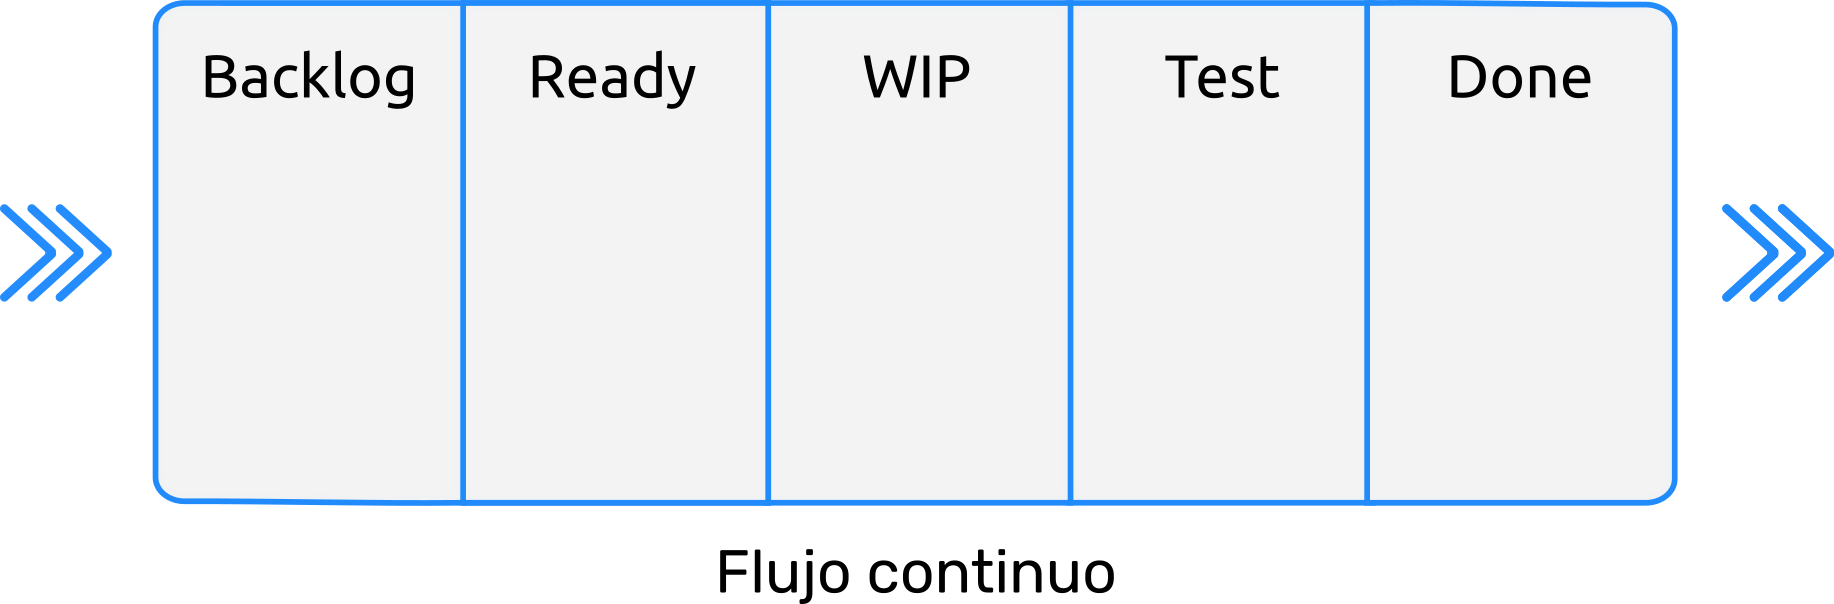
\includegraphics[width=0.8\textwidth]{kanban}
	\caption{Tablero Kanban utilizado.}
\end{figure}

Como herramienta de gestión Kanban, empleamos Kanboard \cite{kanboard}. Se trata de una aplicación \emph{web} \emph{open-source} activamente desarrollada. Contratamos un servidor EC2 con Amazon Web Services (AWS) desde el cual podemos servir la aplicación \emph{web} PHP, la cual a su vez hace uso de una base de datos PostgreSQL en la cual almacena los datos generados. Dicha base de datos está desplegada a través del servicio RDS, también perteneciente a1 AWS.

Se puede acceder al tablero público a través de \href{https://board.jizt.it/public/board/c08ea3322e2876652a0581e79d6430e2dc0c27720d8a06d7853e84c3cd2b}{\texttt{https://kanban.jizt.it}}.

\begin{figure}[h]
	\centering
	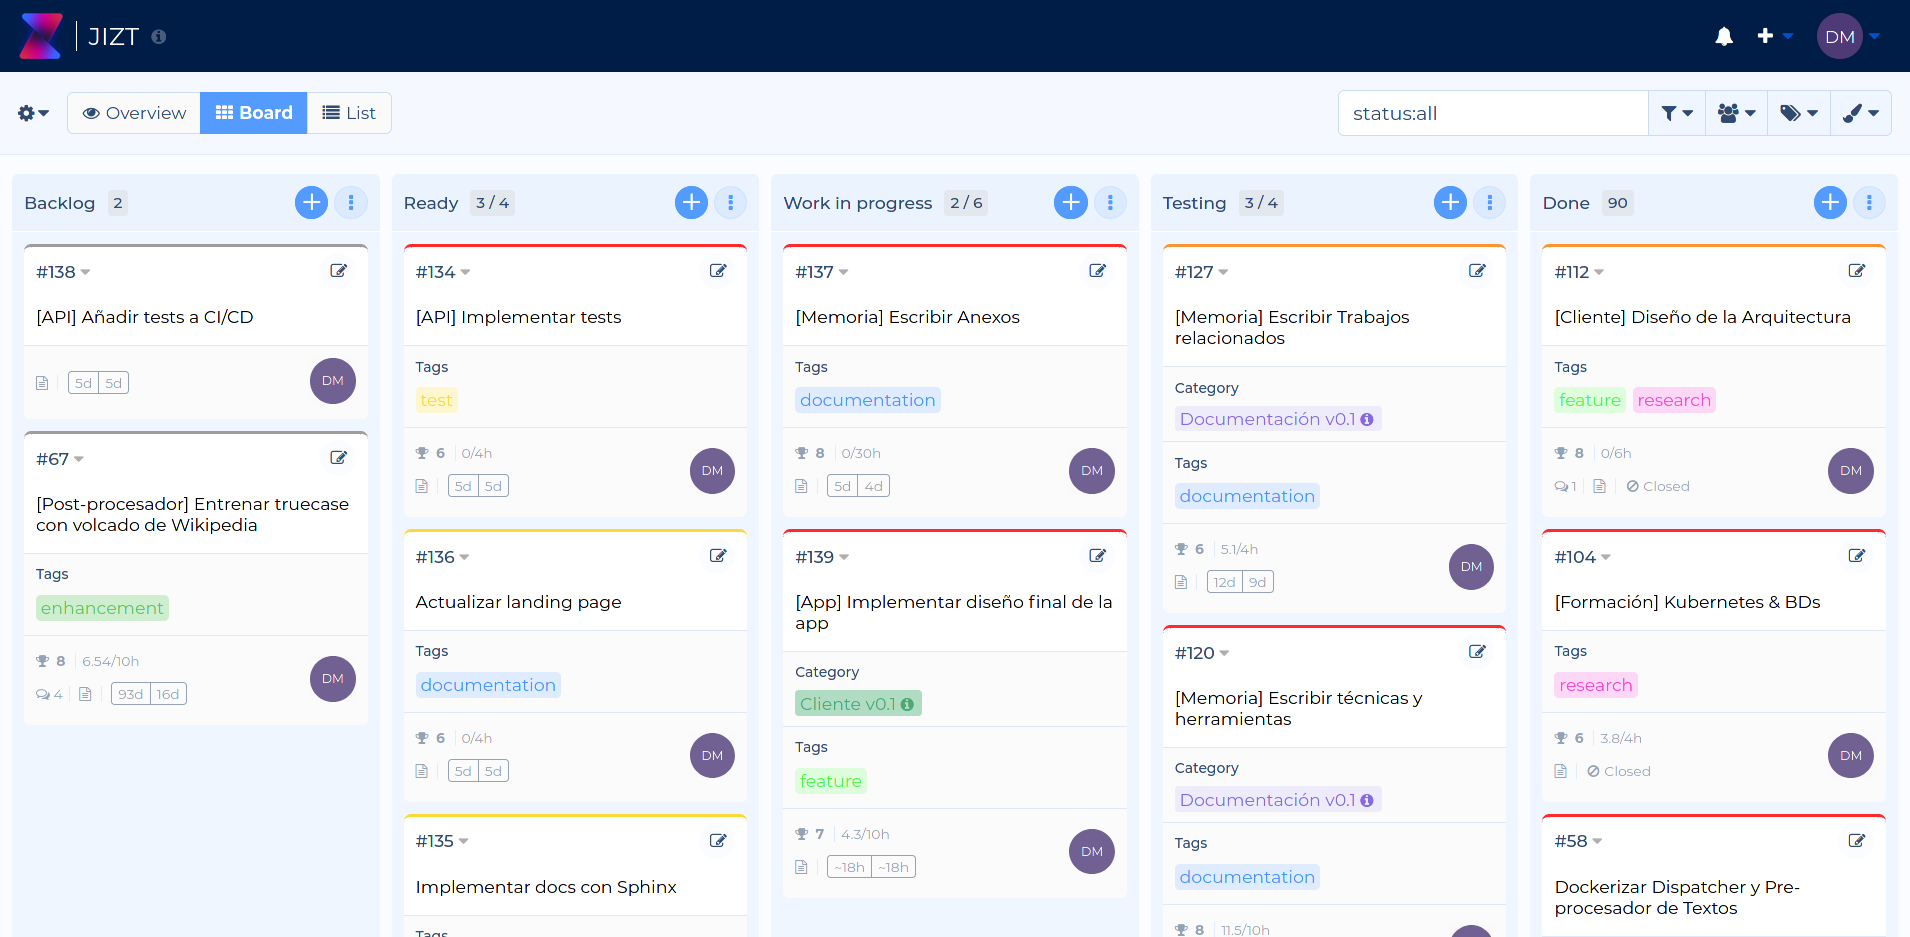
\includegraphics[width=\textwidth]{kanboard}
	\caption[Tablero de Kanboard.]{Captura de pantalla de nuestro tablero Kanban en la aplicación \emph{web} Kanboard.}
\end{figure}


\section{Motivación tras las arquitecturas desarrolladas}

\subsection{Arquitectura de microservicios}

Desde un primer momento, se concibió la arquitectura con los siguientes objetivos presentes:

\vspace{-0.3cm}
\begin{itemize}
	\item [\textbullet] \textbf{Flexibilidad}: la Inteligencia Artificial y, en concreto, el Procesamiento de Lenguaje Natural, son campos en continuo desarrollo. Cada pocos meses aparecen modelos más potentes que proporcionan mejores resultados. Es por ello que nuestra arquitectura debe proporcionar una estructura lo más desacoplada como sea posible de los modelos concretos de NLP que empleados. De este modo, si aparecieran modelos más avanzados, la transición de unos modelos a otros resultará una labor relativamente sencilla.
	\item [\textbullet] \textbf{Escalabilidad}: los elementos que conforman la arquitectura, deben tener la capacidad de replicarse a fin de responder correctamente a la demanda de usuarios. Adicionalmente, como se ha venido mencionado a lo largo de esta memoria, la implementación de otras tareas de NLP diferentes de la generación de resúmenes es algo que entra dentro de nuestros planes a medio plazo. La arquitectura debe estar estructurada de tal forma que esta expansión se pueda llevar a cabo sin inconvenientes. 
	\item [\textbullet] \textbf{Alta disponibilidad}: relacionado con el punto anterior, se debe poder prestar servicio de forma continua, independientemente de que se produzcan picos en la carga de trabajo, o de que alguno de los componentes falle en un momento dado.
	\item [\textbullet] \textbf{\emph{Cloud native}}: este punto engloba a todos los anteriores; los sistemas \emph{cloud-native} están diseñados para adaptarse a entornos cambiantes, operar a gran escala y poseer resiliencia \cite{cloud20}.
\end{itemize}

Una de las arquitecturas que permiten conseguir los objetivos recogidos anteriormente, es la \textbf{arquitectura de microservicios}. Con este patrón arquitectónico, la aplicación se divide en pequeños servicios, cada uno de los cuales cumple una labor específica y encapsula todas sus dependencias, a fin de conseguir el máximo grado de independencia posible.

En nuestro caso, además, existen tareas que llevan considerablemente más tiempo que otras, como es el caso de la generación del resumen (que puede durar segundos), frente al pre-procesado del texto (el cual es instantáneo). Una arquitectura como esta nos permite replicar el microservicio encargado de la generación del resumen, a fin de repartir la carga de trabajo entre las diferentes réplicas. E incluso, podríamos ejecutar los distintos microservicios en máquinas con prestaciones diferentes, de forma que, por ejemplo, el Generador de resúmenes se ejecutara en una máquina más potente, equipada con una GPU, mientras que el resto de microservicios corrieran en máquinas más convencionales. De este modo, reduciríamos los cuellos de botella, manteniendo al mismo tiempo los costes económicos dentro de unos márgenes razonables.

Añadido a todo lo anterior, si uno de los microservicios fallara, sería reemplazado inmediatamente por una nueva réplica, gracias a la tecnología de Kubernetes.

\subsection{Arquitectura dirigida por eventos}

Dado que ya ha sido introducida en la \hyperref[subsec:kafka]{sección referente a Kafka}, no entraremos en mucho detalle para evitar repetirnos.

Simplemente recordaremos que este patrón arquitectónico hace posible la comunicación entre los microservicios de forma fiable y rápida. En nuestro caso, un evento sería la finalización del trabajo por parte de uno de los microservicios. Este evento genera una respuesta en otro de los microservicios, el cual procesa dicho evento y comienza su labor específica.

Este patrón nos ofrece también flexibilidad a la hora de introducir nuevos microservicios, ya que, al menos en el caso de Kafka, el \emph{topic} al que un microservicio produce (o consume) eventos podría ser modificado en tiempo de ejecución, sin necesidad de alterar el código fuente del microservicio.

Finalmente, recordar que el hecho de incrementar el número de réplicas de los microservicios, no influye en el correcto funcionamiento de Kafka, el cual gestiona este escalado de manera transparente.

\subsection{API REST Asíncrona}

La generación de resúmenes es un proceso que se puede dilatar varios segundos en el tiempo, dependiendo de factores como la longitud del texto o de los parámetros con los que se genere el resumen. Por lo tanto, realizar peticiones síncronas queda descartado, puesto que una petición HTTP no debe prolongarse durante tanto tiempo.

La forma común de solucionar este problema, logrando asincronismo, pasa por realizar una primera petición dándole a conocer al sistema que queremos generar un resumen. El sistema, entonces, responderá haciéndonos saber que la petición ha sido recibida y se está procesando. A partir de ese momento, consultaremos periódicamente al servidor para conocer el estado del resumen, hasta finalmente obtenerlo, una vez haya sido generado.

Veamos el proceso de manera un poco más detallada.

\subsubsection{1. Petición HTTP POST}

El cliente comienza realizando una petición POST incluyendo en el cuerpo de la misma el texto que desea resumir. La API le responde con un identificador único del resumen, el \texttt{summary\_id}, así como otros campos de interés:

\begin{figure}[h]
	\centering
	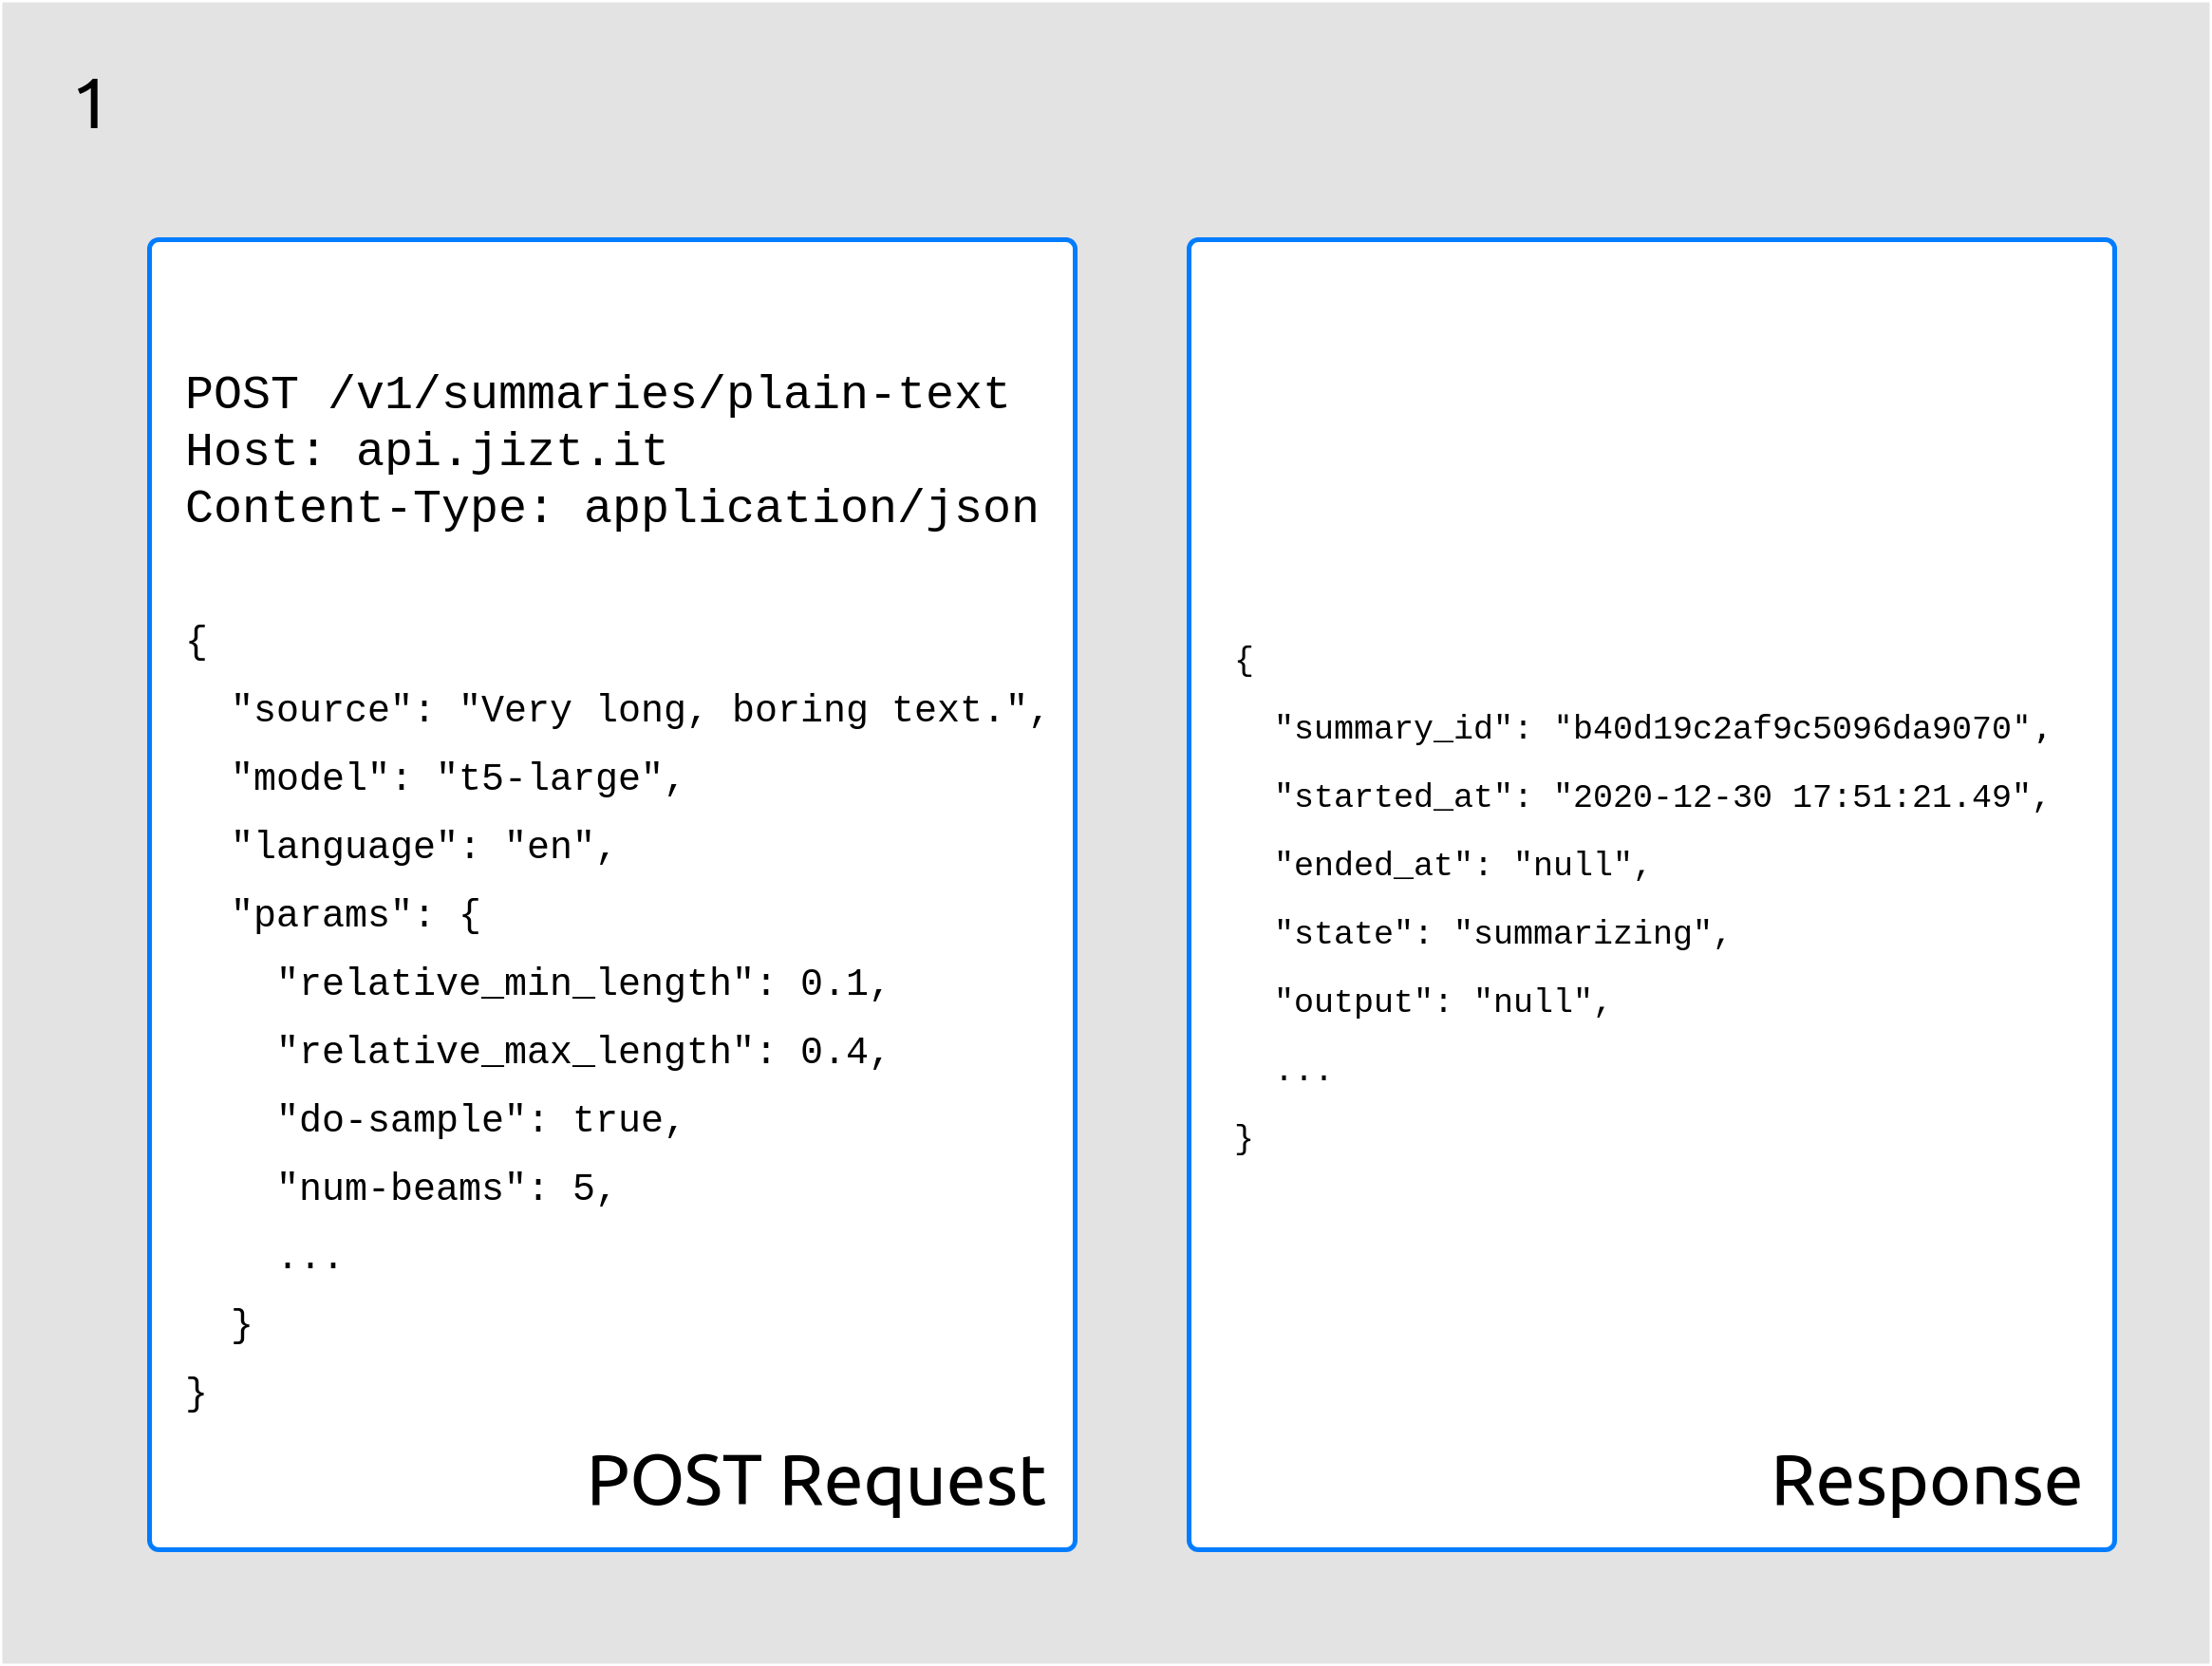
\includegraphics[width=\textwidth]{api-request-1}
	\caption[Primer paso: realizar una petición POST.]{El primer paso es realizar una petición POST con el texto a resumir.}
	\label{fig:api-primer-paso}
\end{figure}

Como vemos en la \autoref{fig:api-primer-paso}, el estado del resumen es \texttt{``resumiendo''} (\texttt{``summarizing''}), y aún no tenemos acceso al resumen (\texttt{ouput}), el cual es por el momento \texttt{``null''}.

Una de las principales ventajas de poder consultar el estado del resumen, es poder ofrecer al usuario retroalimentación de los pasos que se están llevando a cabo, mostrándole así que su resumen efectivamente está siendo procesado.

\subsubsection{2. Peticiones HTTP GET sucesivas}

En ese momento, el cliente puede llevar a cabo peticiones HTTP GET con el \emph{id} del resumen de manera periódica a fin de consultar el estado del mismo.

En algún momento, el estado del resumen pasará a ser \texttt{``completado''} (\texttt{``completed''}), y la respuesta a nuestra petición contendrá el resumen generado, como se ilustra en la \autoref{fig:api-segundo-paso}.

\begin{figure}[h]
	\centering
	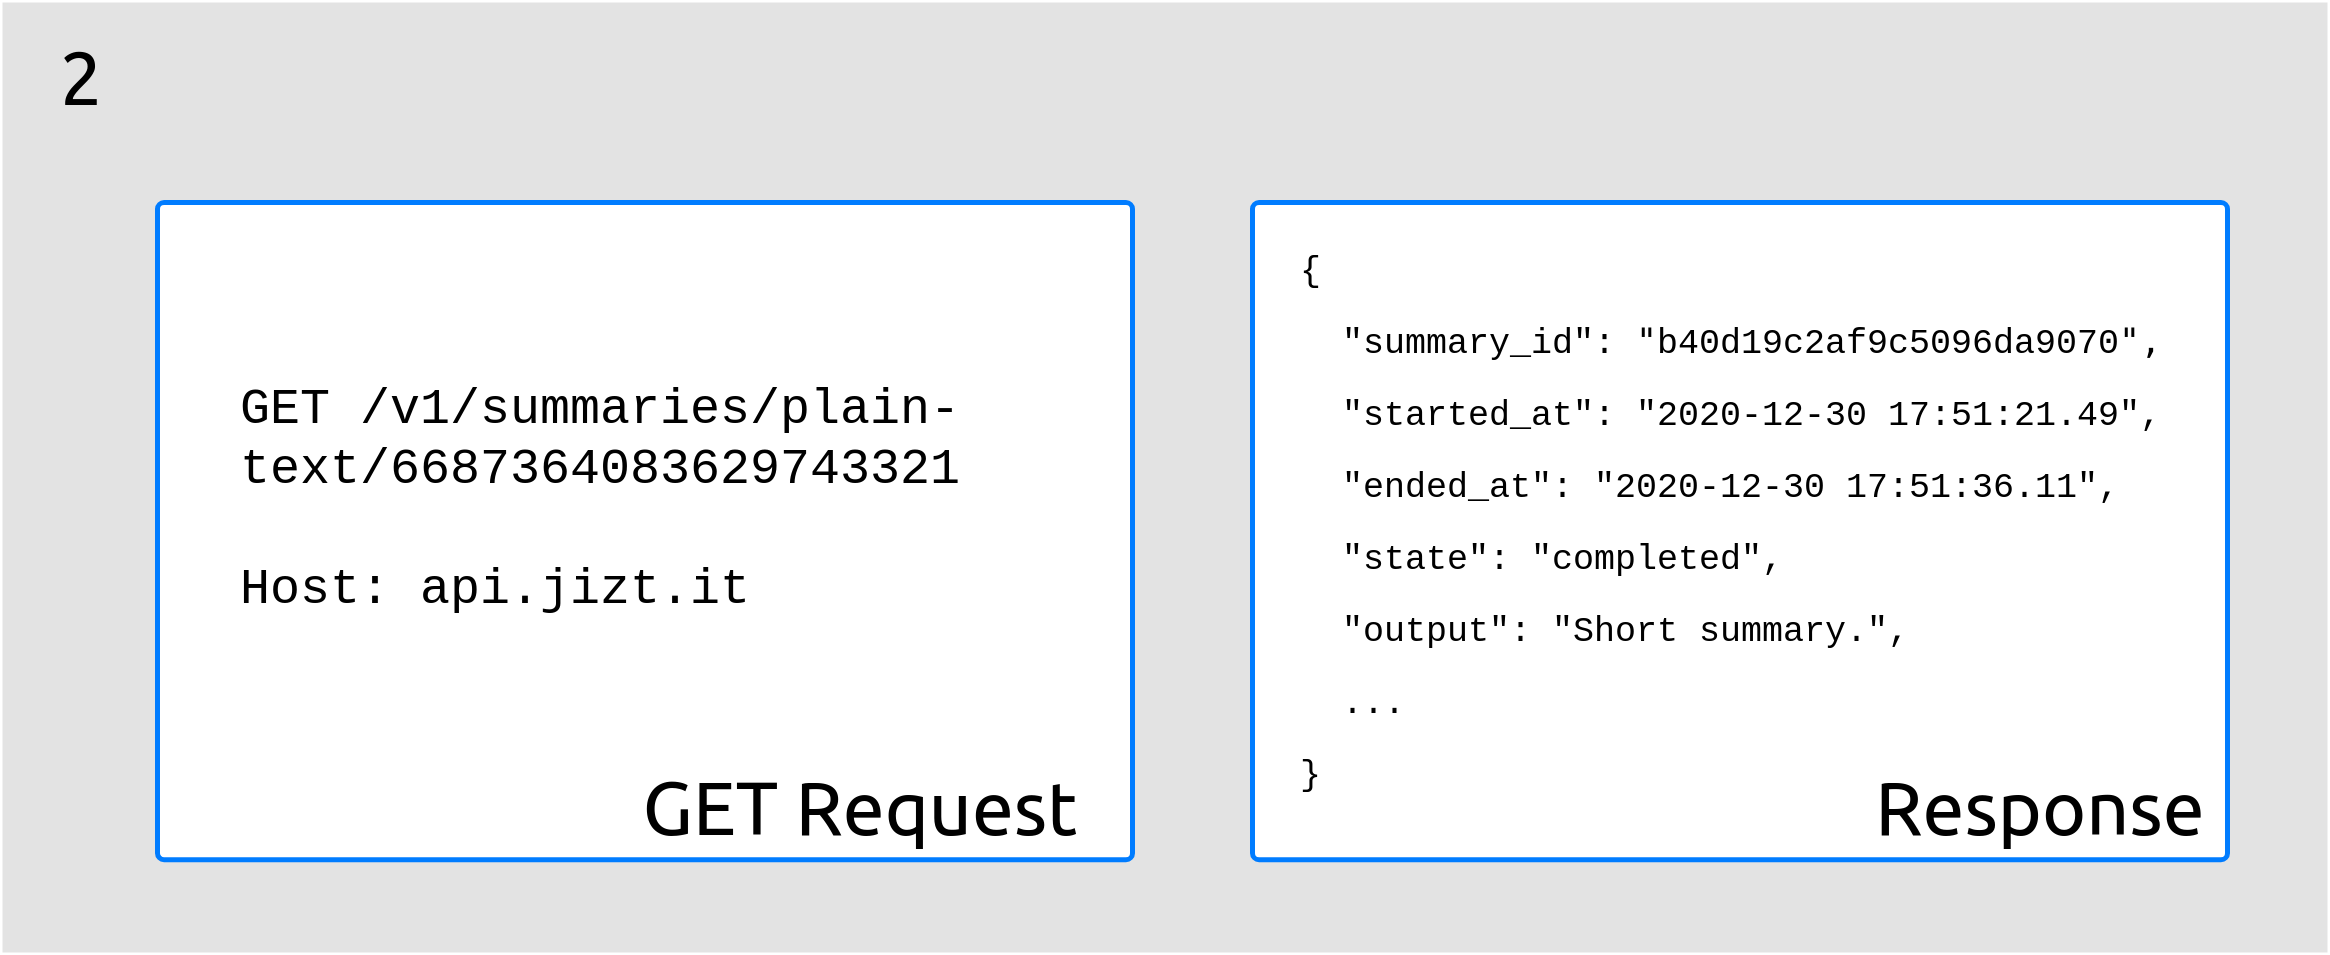
\includegraphics[width=\textwidth]{api-request-2}
	\caption{Finalmente, obtenemos el resumen generado.}
	\label{fig:api-segundo-paso}
\end{figure}

En el caso de que previamente se hubiera solicitado un resumen del mismo texto, con el mismo modelo y parámetros, el resumen ya estaría almacenado en la base de datos, por lo que la respuesta al primer POST ya contendría dicho resumen.

\newpage

\subsection{Desarrollo de la aplicación}

A la hora de desarrollar la aplicación, se ha dado gran importancia al diseño de una aplicación robusta e intuitiva, pero al mismo tiempo fácil de mantener y con capacidad para añadir nuevas funcionalidades.

Con estos objetivos en mente, nos decantamos por implementar una arquitectura de cuatro capas y que se inspira principalmente en los patrones de \emph{Clean Architecture} \cite{martin15} y \emph{Domain-Driven Design} (DDD) \cite{vernon13}.

Como resultado, los principios fundamentales de la arquitectura desarrollada son:

\begin{itemize} [\textbullet]
	\item División del código de la aplicación en capas: cada capa aísla un área de la base de código.
	
	\item Cada capa es estricta con sus dependencias, pudiendo interaccionar únicamente con las capas inferiores.
	
	\item Según se avanza hacia capas inferiores, el código se vuelve más genérico. De este modo, las capas inferiores dictan políticas y reglas, mientras que las capas superiores se encargan de detalles de implementación como bases de datos, operaciones de red o la interfaz de usuario.
	
	\item La estructura y lenguaje del código se deben basar en el dominio de negocio.
\end{itemize}

La \autoref{fig:clean-arch}, ilustra el patrón de \emph{Clean Architecture}, y se puede aplicar asimismo a nuestra arquitectura.

Estos principios nos garantizan que, aunque los requerimientos, tecnologías o la interfaz de usuario de la aplicación cambien con el tiempo, las funcionalidades esenciales de la aplicación no se verán significativamente afectadas. Además, este aislamiento entre capas nos proporciona una mayor escalabilidad y capacidad de testeo de nuestro código.

\begin{figure}[!h]
	\centering
	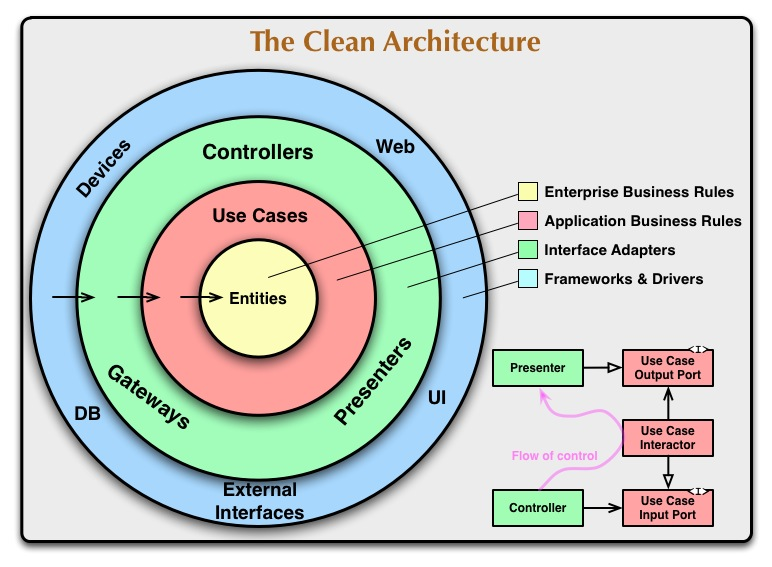
\includegraphics[width=\textwidth]{clean-architecture}
	\caption[Ilustración de \emph{Clean Architecture}.]{Ilustración de \emph{Clean Architecture} \cite{martin15}. La arquitectura se divide en capas, cada una con unas responsabilidades definidas y acotadas.}
	\label{fig:clean-arch}
\end{figure}


La \autoref{fig:app-arch} muestra cómo se conforma la arquitectura de la aplicación. Como podemos ver, las cuatro capas mencionadas en las que se divide nuestra aplicación son: Presentación, Aplicación, Datos y Dominio.

\begin{figure}[!h]
	\centering
	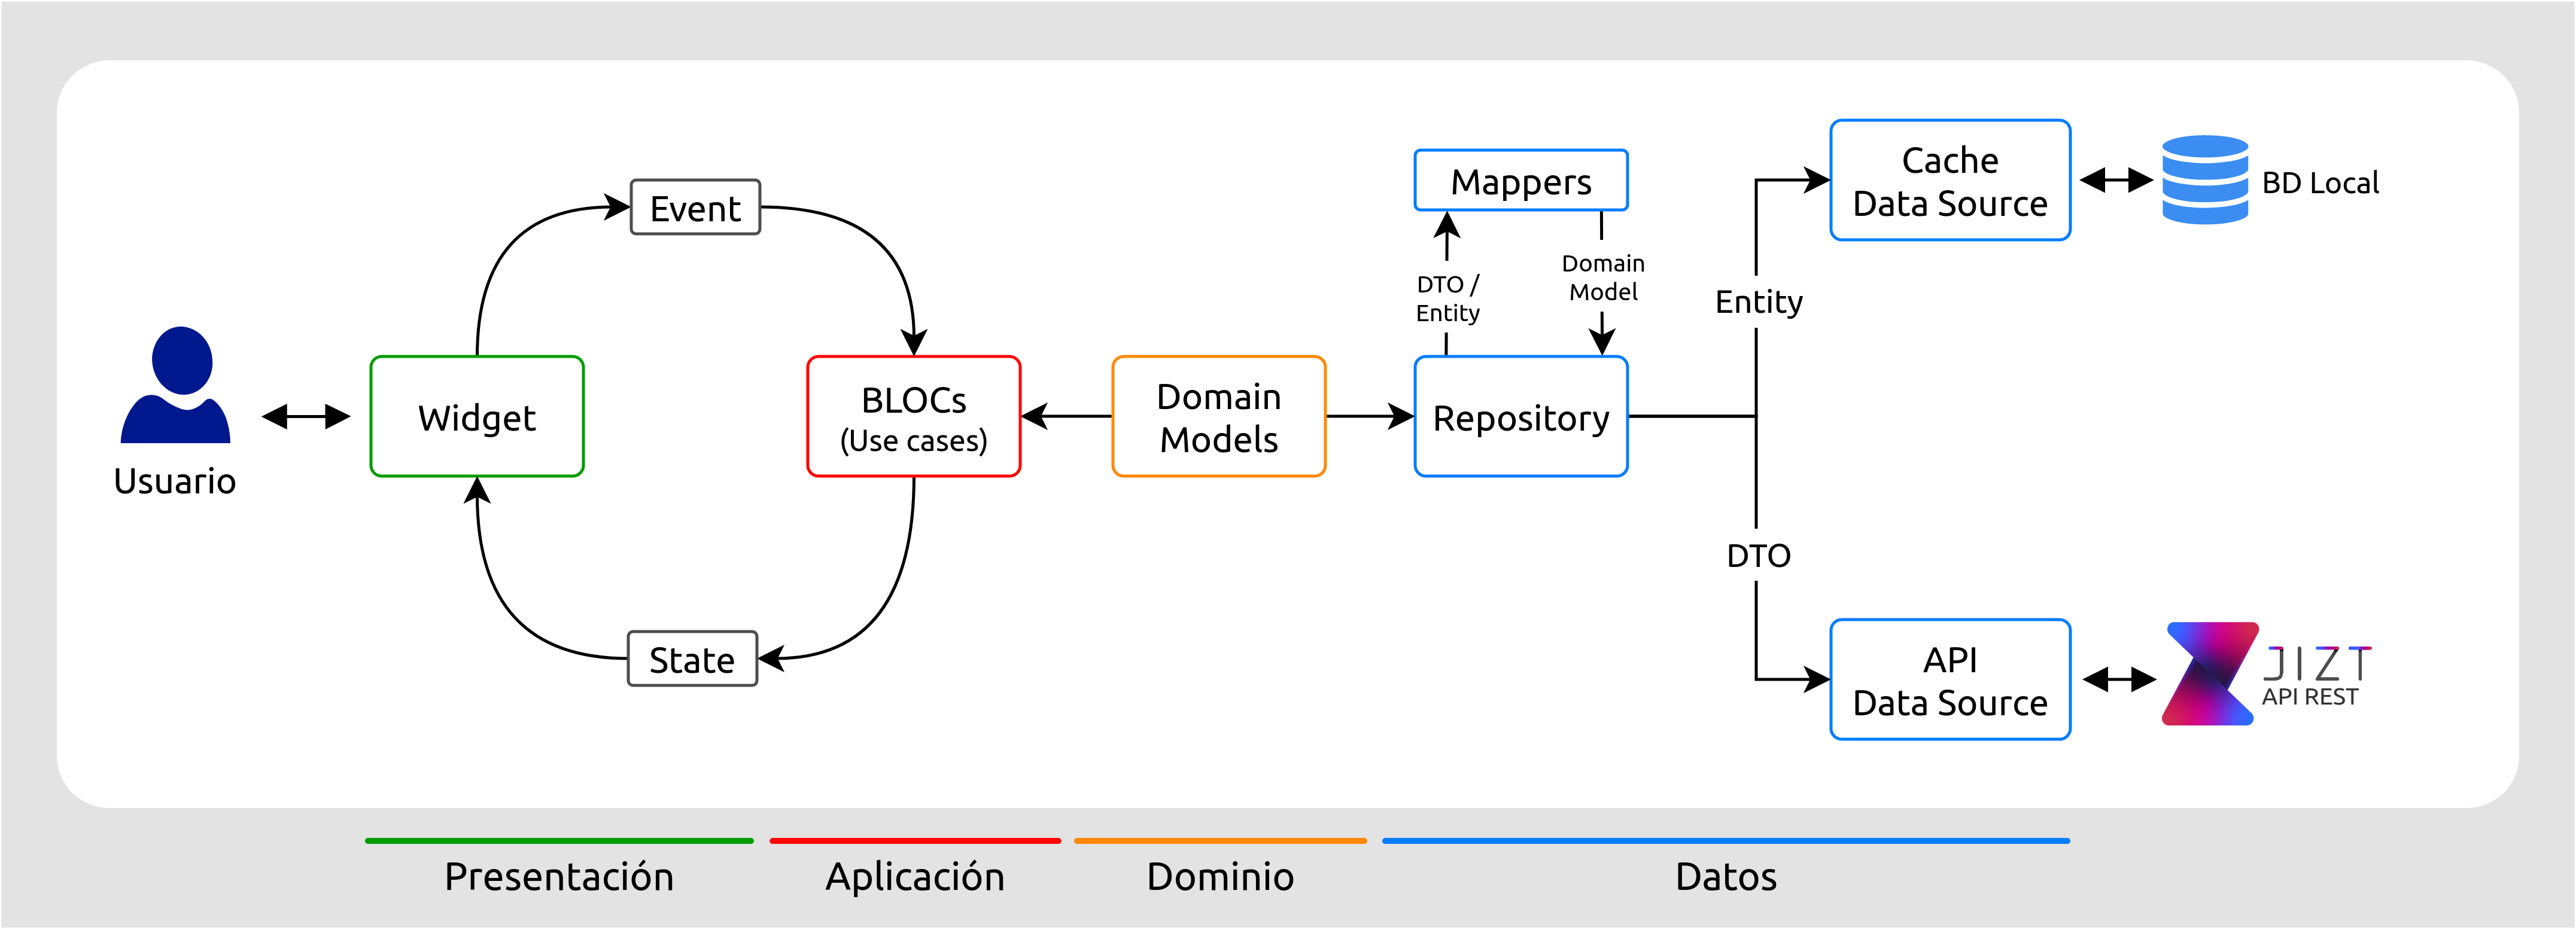
\includegraphics[width=\textwidth]{jizt-app-arch}
	\caption{Arquitectura de la aplicación.}
	\label{fig:app-arch}
\end{figure}

Expliquemos de forma más detallada cada una de ellas, comenzando por la capa de \emph{datos}, a la derecha de la imagen.

\subsubsection{Capa de datos}

La capa de datos es la responsable de persistir y cargar modelos de dominio. En ella se emplea el patrón repositorio, que permite encapsular y centralizar la lógica de acceso a las fuentes de datos, facilitando el mantenimiento y desacoplando el resto de capas de la infraestructura y tecnología que finalmente almacena los datos.

En nuestro caso el repositorio abstrae dos fuentes de datos:

\vspace{-0.3cm}
\begin{itemize} [\textbullet]
	\item Fuente de datos remota: consume la API REST del \emph{backend}.
	
	\item Fuente de datos local: se emplea una base de datos local como caché para almacenar los resúmenes generados. Esto permite al usuario acceder a su historial de resúmenes.
\end{itemize}

Además de centralizar el acceso a datos, el repositorio también es responsable de transformar las diferentes representaciones de los modelos de dominio con los que trabaja la aplicación utilizando lo que se conoce como \emph{mappers}. Dichos representaciones son:

\vspace{-0.3cm}
\begin{itemize} [\textbullet]
	\item Modelo de dominio (\emph{domain model}): es la representación de los datos a través de la estructura más apropiada para la aplicación junto con sus reglas de negocio.
	\item DTO (\emph{Data Transfer Object}): se corresponde con la representación de los datos en los documentos JSON que se envían y reciben de la API REST. Su estructura es la más adecuada para la comunicación remota.
	\item Entidad de la base de datos (\emph{database entity}): es la representación de los datos en la base datos local. Su estructura es la más adecuada para persistir la información en dicha base de datos.
\end{itemize}

Como consecuencia, el hecho de separar los modelos en estas tres representaciones diferentes nos permite:

\vspace{-0.3cm}
\begin{itemize} [\textbullet]
	\item Encapsular en los DTOs todas las anotaciones específicas del \emph{framework} que nos permite serializar y deserializar los documentos JSON.
	
	\item Encapsular en las \emph{database entities} todas las anotaciones que nos permiten almacenar objetos en la base de datos.
	
	\item Mantener los \emph{domain models} independientes de cualquier \emph{frameworks} específico. De este modo, si en un futuro se reemplaza, por ejemplo, el \emph{framework} de serialización de los documentos JSON, la capa de dominio no se vería afectada.
	
	\item Cachear localmente la información realmente necesaria (por ejemplo, prescindiendo de algunos metadatos que devuelve la API REST y que no son relevantes para el usuario de la aplicación, o almacenando información adicional que no devuelve la API).
\end{itemize}


\begin{figure}[!h]
	\centering
	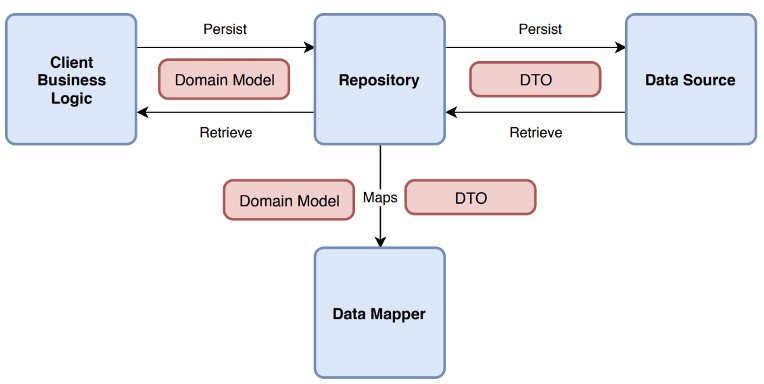
\includegraphics[width=0.9\textwidth]{repository-pattern}
	\caption[Patrón repositorio.]{Patrón repositorio \cite{brandi19}. En esta imagen se ilustran los diferentes dominios explicados, así como la transformación de los modelos de unos dominios a otros por parte del \emph{Data Mapper}.}
\end{figure}

\subsubsection{Capa de dominio}

Esta capa define la lógica de dominio de la aplicación, y es independiente de la plataforma de desarrollo, es decir, en nuestro caso estará escrita puramente en Dart, sin contener ningún elemento de Flutter \cite{flutter-clean-arch}. El motivo reside en que el dominio, como decíamos, solo debe ocuparse de la lógica de negocio, y no de los detalles de implementación. Esto también permite una fácil migración entre plataformas, en caso de ser necesario en algún momento.

La capa de dominio contiene los \emph{domain models} que representan los conceptos de negocio junto con sus reglas.

Además de los \emph{domain models}, esta capa contiene las definiciones (interfaces) de los repositorios implementados en la capa de datos. A través de esta técnica, conocida como inversión de dependencias (\emph{dependency inversion}), se logra mantener la capa de dominio totalmente independiente de las demás capas y de los \emph{frameworks} que estas usan (por ejemplo, Flutter en la capa de presentación o Hive\footnote{\, Hive es un paquete para Flutter que permite implementar bases de datos clave-valor. En nuestro caso, lo empleamos para almacenar los resúmenes localmente.} en la capa de datos), limitando su ámbito estrictamente a la representación de los conceptos de negocio junto con sus reglas.

\subsubsection{Capa de aplicación}

La capa de aplicación contiene toda la lógica de negocio de aplicación (\emph{application business logic}, no confundir con la \emph{domain business logic de} la capa de dominio). Esta se encarga principalmente de orquestar el resto de capas.

En ella utilizamos el patrón BLoC (Business Logic Component) \cite{miola20}, se basado en dos elementos principales: eventos y estados.

Desde fuera podemos imaginarnos un BLoC como una caja negra a la que se le proporcionan eventos como entrada (por ejemplo ``cargar todos los resúmenes'') y el BLoC emite un estado como salida (en el ejemplo anterior, el nuevo estado incluiría la lista de resúmenes).

En el interior del BLoC se encuentra la lógica de negocio de aplicación que, dado un evento de entrada, acudirá a la capa de dominio para recuperar, guardar o validar información, y finalmente actualizará el estado según el resultado de esas operaciones.

\subsubsection{Capa de presentación}

La capa de presentación es la más cercana al usuario y se encarga de dibujar la interfaz de usuario, así como de propagar las interacciones del usuario a la capa de aplicación. No posee ninguna lógica de negocio; únicamente presenta lógica de presentación (por ejemplo, cómo pintar un botón dependiendo de su estado, cómo navegar entre pantallas, cómo ejecutar una animación, etc.).

En esta capa encontramos todo el código específico de Flutter, especialmente los \emph{widgets} que componen las vistas finales de la interfaz \cite{flutter-widget}, como un botón o un \emph{layout}. Los \emph{widgets} se organizan de forma jerárquica, de modo que toda aplicación tendrá un \emph{widget} raíz, del cual <<colgarán>> el resto de \emph{widgets}, como podemos ver en la siguiente figura:

\begin{figure}[h!]
	\centering
	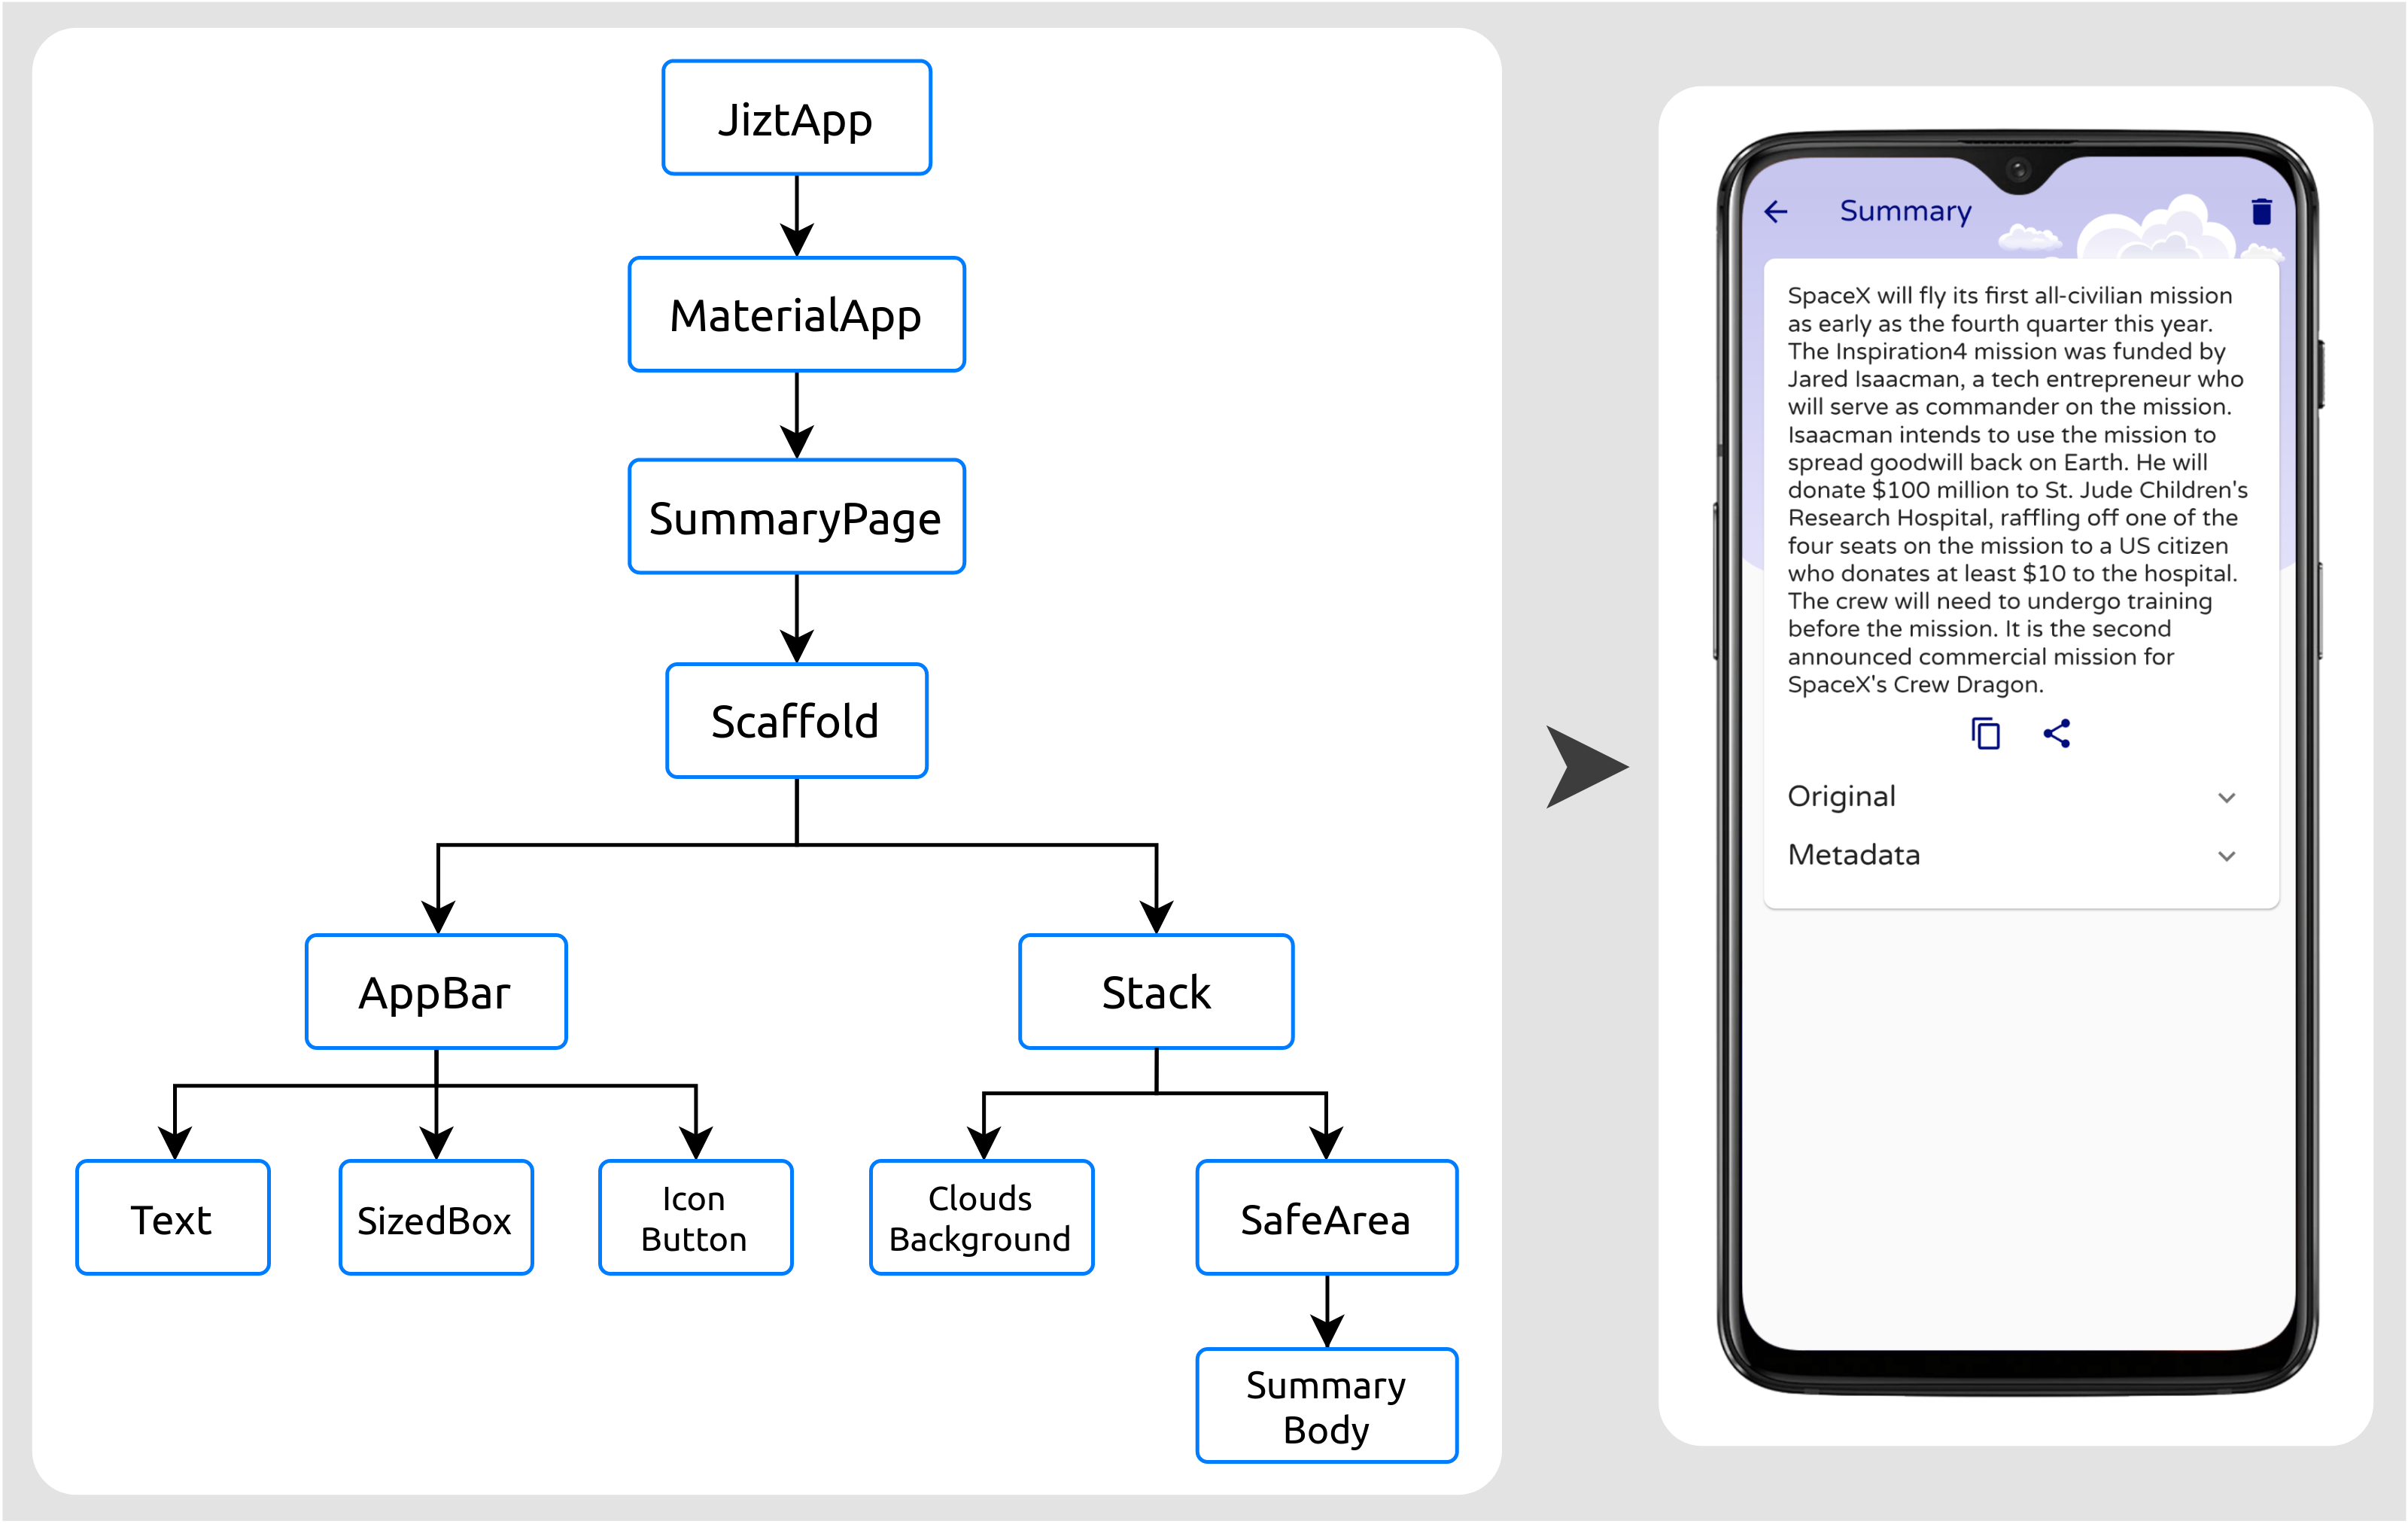
\includegraphics[width=\textwidth]{widget-hierarchy}
	\caption[Ejemplo de jerarquía de \emph{widgets}.]{Ejemplo de jerarquía de \emph{widgets} de una aplicación sencilla. Imagen del dispositivo móvil extraída de \cite{miola20}.}
	\label{flutter-widgets}
\end{figure}

Las interacciones del usuario se propagan como eventos a los BLoC de la capa de aplicación, y estos actualizan su estado acordemente. La capa de presentación <<escucha>> dichos estados y, cada vez que estos cambian, vuelve a dibujar los \emph{widget}, actualizando la pantalla. Cabe mencionar que Flutter realiza esta operación de una forma muy optimizada, volviendo a dibujar solamente aquellas partes de la interfaz que han sido modificadas.


\subsection{Integración y despliegue continuos (CI/DC)}

A fin de seguir buenas prácticas en el entorno de DevOps, hemos implementado integración y despliegue continuos tanto del \emph{backend}, como de la aplicación.

Anteriormente, el uso de estas técnicas se llevaba a cabo a través de herramientas de automatización como Jenkins \cite{jenkins} o Travis CI \cite{travis}.

No obstante, GitHub (en el cual alojamos nuestros repositorios del proyecto) ha lanzado recientemente su propio servicio con este fin, llamado GitHub Actions \cite{github-actions}, que permite implementar CI/CD directamente desde esta plataforma, sin tener que hacer uso de aplicaciones de terceros. Esta ha sido, por tanto, la opción escogida en nuestro caso.

Una de las grandes ventajas de GitHub Actions reside en que existen <<acciones>> predefinidas y reutilizables, escritas previamente por otros usuarios, que llevan a cabo tareas comunes o rutinarias. De este modo, no necesitamos encargarnos de, por ejemplo, lidiar con todos los detalles específicos para poder conectarnos a nuestro \emph{clúster} en Google Cloud desde GitHub Actions, a fin de poder desplegar el \emph{backend} de forma automática.

Resumamos los principales aspectos del CI/CD en el caso del \emph{backend} y de la aplicación, los cuales se alojan en dos repositorios diferentes.

\subsubsection{CI/CD en el repositorio del \emph{backend}}

En el caso del \emph{backend}, hemos reservado la rama \texttt{main} como rama principal de producción. Por tanto, siempre que trabajamos sobre alguna mejora o cambio, creamos una nueva para ello. Cuando hemos finalizado de implementar esos cambios, hacemos un \emph{merge} con la rama principal.

En el momento que esto ocurre, se ponen en funcionamiento las tareas de GitHub Actions. Lo primero que se lleva a cabo es una ejecución automática de los \emph{tests} desarrollados para la prueba del \emph{backend}. Solo en el caso de que todos los \emph{tests} hayan sido exitosos, se procede a desplegar la nueva versión del \emph{backend} en nuestro \emph{clúster} de producción de Google Kubernetes Engine (GKE). Esta actualización se realiza sin tiempos de interrupción, gracias a las ventajas que ofrecen Kubernetes y Helm, ya explicadas con anterioridad.

\bigskip
\noindent
\textbf{DeepSource - Revisión automatizada del código}

Además de los \emph{tests} implementados, hacemos uso de una herramienta llamada DeepSource \cite{deepsource}. Esta herramienta lleva a cabo análisis estáticos de nuestro código, detectando cualquier posible error de sintaxis, anti-patrones, problemas potenciales de seguridad, recomendaciones de estilo, etc.

Hablando personalmente, queremos destacar que la potencia de DeepSource nos ha sorprendido, dado que es capaz de detectar hasta los detalles más sutiles, y por tanto nos ha sido de gran ayuda a la hora de potenciar la calidad de nuestro código.

Se puede hacer uso de DeepSource de manera gratuita durante seis meses con el \emph{pack} de estudiante de GitHub \cite{gh-student-pack}.

\begin{figure}[h!]
	\centering
	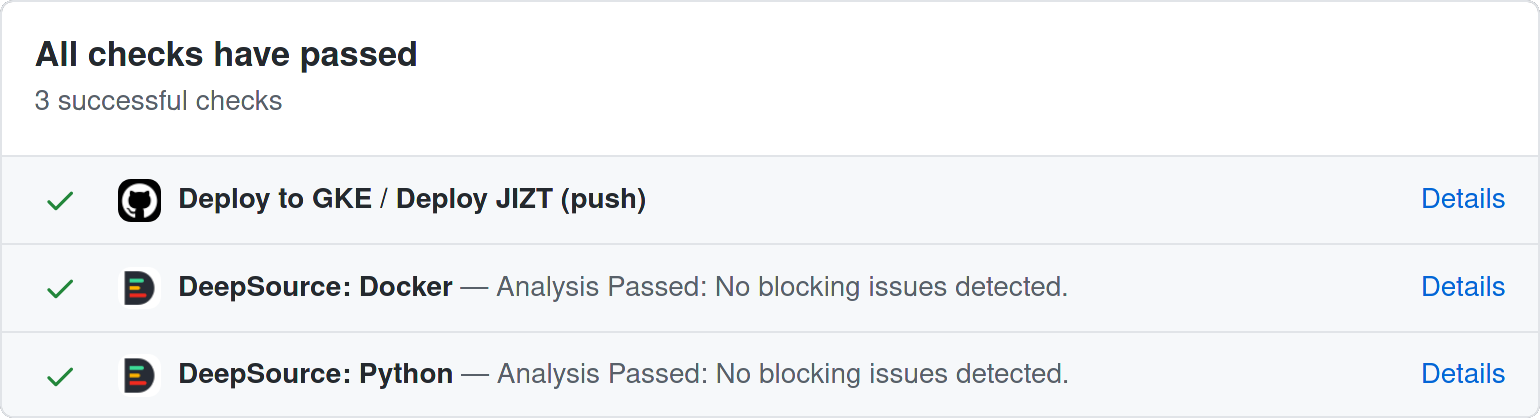
\includegraphics[width=\textwidth]{checks-backend}
	\caption[GitHub Actions.]{Tareas llevadas a cabo cada vez que hacemos un \emph{commit} a la rama \texttt{main} del repositorio. Imagen extraída de GitHub.}
\end{figure}

El repositorio en GitHub correspondiente al \emph{backend} es accesible a través de \href{https://github.com/dmlls/jizt}{https://github.com/dmlls/jizt}.

\subsubsection{CI/CD en el repositorio de la aplicación}

Para la aplicación, también hacemos uso de GitHub Actions para implementar el CI/CD de la misma.

En este caso, se llevan a cabo tres tareas principales:

\vspace{-0.3cm}
\begin{itemize} [\textbullet]
	\item QA: cada vez que se hace un \emph{push} desde cualquier rama se ejecutan los test, se comprueba que el código está correctamente formateado, y se realiza un análisis estático del código. Solo si estas comprobaciones son exitosas se llevará a cabo el \emph{merge} de dicha rama con la rama principal (\texttt{main}).
	
	\item Despliegue de la \emph{web app}: cada vez que la rama principal es actualizada, se compila la nueva versión, y se despliega a GitHub Pages de manera automática.
	
	\item Despliegue de la \emph{app} Android: la estrategia de despliegue que seguimos con la \emph{web} no es ideal para aplicaciones nativas que se distribuyen a través de una \emph{store} (por ejemplo, Play Store), ya que generaría actualizaciones constantemente. Por este motivo utilizamos \emph{tags} de GitHub, que nos permiten lanzar actualizaciones que agrupan varios \emph{commits}. Cada vez que se crea una nueva \emph{tag} (por ejemplo, \texttt{v0.1.1}), se compila la nueva versión de la aplicación de Android y se propaga automáticamente a Google Play.
\end{itemize}

TODO: añadir captura de los checks de GitHub.

Se puede acceder al repositorio correspondiente a la aplicación de JIZT en \href{https://github.com/dmlls/jizt-app}{https://github.com/dmlls/jizt-app}.

\subsection{Distribución de la aplicación}

La distribución de la aplicación se lleva a cabo a través de GitHub y, en su versión Android, también a través de Google Play.

\subsubsection{GitHub}

Cada vez que se produce una nueva versión de la aplicación, se crea una nueva \emph{Release} en GitHub que contiene el código fuente de la aplicación.

TODO: desarrollar un poco más, añadir alguna captura.

\bigskip
\noindent
\textbf{{\small GitHub Pages}}

GitHub Pages es un servicio de \emph{hosting} para páginas \emph{web} estáticas que nos permite servir nuestra aplicación en su versión \emph{web} de manera gratuita.

Se puede acceder a la aplicación de JIZT a través de \href{https://app.jizt.it}{https://app.jizt.it}.

En nuestro caso, también hacemos uso de este servicio para alojar la \emph{landing page} del proyecto (\href{https://www.jizt.it}{https://www.jizt.it}), así como la documentación del proyecto (\href{https://docs.jizt.it}{https://docs.jizt.it}), y la documentación de la API REST (\href{https://docs.api.jizt.it}{https://docs.api.jizt.it}).

\subsubsection{Play Store}

La aplicación, en su versión Android, también está disponible a través de Play Store, de momento únicamente a través del programa \emph{Internal Early Access}. Esto significa que únicamente aquellos usuarios que dispongan del \emph{link} podrán hacer uso de ella.

TODO: añadir link.

En las próximas semanas, se publicará la primera versión estable de la aplicación.

TODO: añadir captura Google Play.


\subsection{Limitaciones económicas del proyecto}

Por último, creemos conveniente mencionar uno de los principales inconvenientes del proyecto desarrollado. Por introducirlo de manera rápida y sencilla: la contratación de servidores en la nube no es gratuita.

Para desplegar toda nuestra infraestructura de microservicios, y escalarla de forma que podamos atender a un alto volumen de usuarios, necesitaríamos aumentar el número de nodos en nuestro \emph{clúster} de Kubernetes, lo cual incrementaría significativamente los costes.

Actualmente, hacemos uso del servicio Google Kubernetes Engine (GKE) de Google Cloud, y disponemos de un único \emph{clúster} de Kubernetes con un solo nodo que ejecuta una máquina de tipo ``e2-standard-4'', la cual cuenta con 4 CPUs virtuales y 16 GB de RAM. No obstante, un despliegue mínimo de la aplicación hace uso de tan solo 1,32 GB de RAM.

No nos vamos a engañar: el elevado coste de estos servicios es una de las principales amenazas de la continuación del proyecto.

Por ahora, tenemos capacidad para mantenernos algunos meses más (3 o 4, calculamos), con los créditos gratuitos que ofrecen \emph{cloud providers} como Google Cloud o Amazon Web Services (AWS).

Por hacernos una idea de la magnitud de los costes, Google Cloud nos ofreció un crédito gratuito de 273 €, los cuales se habrán consumido en las próximas dos o tres semanas.

Actualmente, estamos pensando en alternativas para la financiación del proyecto, aunque creemos que por ahora la única solución a corto plazo pasa por confiar en posibles donaciones puntuales y en los créditos gratuitos de los diferentes \emph{cloud providers}.

Asimismo, otra alternativa pasa por ofrecer un servicio de despliegue de la infraestructura desarrollada en este proyecto para terceras partes (instituciones, empresas, particulares, etc.) que pudieran estar interesadas. Con la contratación de este servicio, nos encargaríamos de atender todos los detalles de instalación, puesta en marcha y mantenimiento del sistema. El despliegue se podría hacer tanto a través de un \emph{cloud provider} como en las dependencias propias del interesado.